\documentclass[10pt, french]{article}

%% -----------------------------
%% Préambule
%% -----------------------------
% !TEX encoding = UTF-8 Unicode
% LaTeX Preamble for all cheatsheets
% Author : Gabriel Crépeault-Cauchon

% HOW-TO : copy-paste this file in the same directory as your .tex file, and add in your preamble the next command right after you have specified your documentclass : 
% \input{preamble-cheatsht.tex}
% ---------------------------------------------
% ---------------------------------------------

% Extra note : this preamble creates document that are meant to be used inside the multicols environment. See the documentation on internet for further information.

%% -----------------------------
%% Encoding packages
%% -----------------------------
\usepackage[utf8]{inputenc}
\usepackage[T1]{fontenc}
\usepackage{babel}
\usepackage{lmodern}

%% -----------------------------
%% Variable definition
%% -----------------------------
\def\auteur{Gabriel Crépeault-Cauchon / Nicholas Langevin}
\def\BackgroundColor{white}

%% -----------------------------
%% Margin and layout
%% -----------------------------
% Determine the margin for cheatsheet
\usepackage[landscape, hmargin=1cm, vmargin=1.7cm]{geometry}
\usepackage{multicol}

% Remove automatic indentation after section/subsection title.
\setlength{\parindent}{0cm}

% Save space in cheatsheet by removing space between align environment and normal text.
\usepackage{etoolbox}
\newcommand{\zerodisplayskips}{%
  \setlength{\abovedisplayskip}{0pt}%
  \setlength{\belowdisplayskip}{0pt}%
  \setlength{\abovedisplayshortskip}{0pt}%
  \setlength{\belowdisplayshortskip}{0pt}}
\appto{\normalsize}{\zerodisplayskips}
\appto{\small}{\zerodisplayskips}
\appto{\footnotesize}{\zerodisplayskips}

%% -----------------------------
%% URL and links
%% -----------------------------
\usepackage{hyperref}
\hypersetup{colorlinks = true, urlcolor = gray!70!white, linkcolor = black}

%% -----------------------------
%% Document policy (uncomment only one)
%% -----------------------------
%	\usepackage{concrete}
	\usepackage{mathpazo}
%	\usepackage{frcursive} %% permet d'écrire en lettres attachées
%	\usepackage{aeguill}
%	\usepackage{mathptmx}
%	\usepackage{fourier} 

%% -----------------------------
%% Math configuration
%% -----------------------------
\usepackage[fleqn]{amsmath}
\usepackage{amsthm,amssymb,latexsym,amsfonts}
\usepackage{empheq}
\usepackage{numprint}
\usepackage{dsfont} % Pour avoir le symbole du domaine Z

% Mathematics shortcuts

\newcommand{\reels}{\mathbb{R}}
\newcommand{\entiers}{\mathbb{Z}}
\newcommand{\naturels}{\mathbb{N}}
\newcommand{\eval}{\biggr \rvert}
\usepackage{cancel}
\newcommand{\derivee}[1]{\frac{\partial}{\partial #1}}
\newcommand{\prob}[1]{\Pr \left( #1 \right)}
\newcommand{\esp}[1]{\mathrm{E} \left[ #1 \right]} % espérance
\newcommand{\variance}[1]{\mathrm{Var} \left( #1   \right)}
\newcommand{\covar}[1]{\mathrm{Cov} \left( #1   \right)}
\newcommand{\laplace}{\mathcal{L}}
\newcommand{\deriv}[2][]{\frac{\partial^{#1}}{\partial #2^{#1}}}
\newcommand{\e}[1]{\mathrm{e}^{#1}}
\newcommand{\te}[1]{\text{exp}\left\{#1\right\}}
\DeclareMathSymbol{\shortminus}{\mathbin}{AMSa}{"39}



% To indicate equation number on a specific line in align environment
\newcommand\numberthis{\addtocounter{equation}{1}\tag{\theequation}}

%
% Actuarial notation packages
%
\usepackage{actuarialsymbol}
\usepackage{actuarialangle}

%
% Matrix notation for math symbols (\bm{•})
%
\usepackage{bm}
% Matrix notation variable (bold style)
\newcommand{\matr}[1]{\mathbf{#1}}



%% -----------------------------
%% tcolorbox configuration
%% -----------------------------
\usepackage[most]{tcolorbox}
\tcbuselibrary{xparse}
\tcbuselibrary{breakable}

%%
%% Coloured box "definition" for definitions
%%
\DeclareTColorBox{definition}{ o }				% #1 parameter
{
	colframe=blue!60!green,colback=blue!5!white, % color of the box
	breakable, 
	pad at break* = 0mm, 						% to split the box
	title = {#1},
	after title = {\large \hfill \faBook},
}
%%
%% Coloured box "definition2" for definitions
%%
\DeclareTColorBox{definitionNOHFILL}{ o }				% #1 parameter
{
	colframe=blue!60!green,colback=blue!5!white, % color of the box
	pad at break* = 0mm, 						% to split the box
	title = {#1},
	before title = {\faBook \quad },
	breakable
}


%%
%% Coloured box "algo" for algorithms
%%
\newtcolorbox{algo}[ 1 ]
{
	colback = blue!5!white,
	colframe = blue!75!black,
	title=#1,
	fonttitle = \bfseries,
	breakable
}
%%
%% Coloured box "conceptgen" for points adding to a concept's deifintion
%%
\newtcolorbox{conceptgen}[ 1 ]
{
	breakable,
	colback = beaublue,
	colframe = airforceblue,
	title=#1,
	fonttitle = \bfseries
}
%%
%% Coloured box "probch3" pour formules relatives au 3ème chapitre de prob
%%
\newtcolorbox{probch3}[ 1 ]
{
	colback = ruddypink,
	colframe = burgundy,
	fonttitle = \bfseries,	
	breakable,
	title=#1
}
%%
%% Coloured box "formula" for formulas
%%
\newtcolorbox{formula}[ 1 ]
{
	colback = green!5!white,
	colframe = green!70!black,
	breakable,
	fonttitle = \bfseries,
	title=#1
}
%%
%% Coloured box "formula" for formulas
%%
\DeclareTColorBox{algo2}{ o }
{
	enhanced,
	title = #1,
	colback=blue!5!white,	
	colbacktitle=blue!75!black,
	fonttitle = \bfseries,
	breakable,
	boxed title style={size=small,colframe=arsenic} ,
	attach boxed title to top center = {yshift=-3mm,yshifttext=-1mm},
}
%%
%% Coloured box "examplebox" for formulas
%%
\newtcolorbox{examplebox}[ 1 ]
{
	colback = lightmauve,
	colframe = antiquefuchsia,
	breakable,
	fonttitle = \bfseries,title=#1
}
%%
%% Coloured box "rappel" pour rappel de formules
%%
\newtcolorbox{rappel}[ 1 ]
{
	colback = ashgrey,
	colframe = arsenic,
	breakable,
	fonttitle = \bfseries,title=#1
}
%%
%% Coloured box "rappel" pour rappel de formules
%%
\DeclareTColorBox{rappel_enhanced}{ o }
{
	enhanced,
	title = #1,
	colback=ashgrey, % color of the box
%	colframe=blue(pigment),
%	colframe=arsenic,	
	colbacktitle=arsenic,
	fonttitle = \bfseries,
	breakable,
	boxed title style={size=small,colframe=arsenic} ,
	attach boxed title to top center = {yshift=-3mm,yshifttext=-1mm},
}
%%
%% Coloured box "notation" for notation and terminology
%%
\DeclareTColorBox{distributions}{ o }			% #1 parameter
{
	enhanced,
	title = #1,
	colback=gray(x11gray), % color of the box
%	colframe=blue(pigment),
	colframe=arsenic,	
	colbacktitle=aurometalsaurus,
	fonttitle = \bfseries,
	boxed title style={size=small,colframe=arsenic} ,
	attach boxed title to top center = {yshift=-3mm,yshifttext=-1mm},
	breakable
%	left=0pt,
%  	right=0pt,
%    box align=center,
%    ams align*
%  	top=-10pt
}

%% -----------------------------
%% Graphics and pictures
%% -----------------------------
\usepackage{graphicx}
\usepackage{pict2e}
\usepackage{tikz}

%% -----------------------------
%% insert pdf pages into document
%% -----------------------------
\usepackage{pdfpages}

%% -----------------------------
%% Color configuration
%% -----------------------------
\usepackage{color, soulutf8, colortbl}


%
%	Colour definitions
%
\definecolor{blue(munsell)}{rgb}{0.0, 0.5, 0.69}
\definecolor{blue(matcha)}{rgb}{0.596, 0.819, 1.00}
\definecolor{blue(munsell)-light}{rgb}{0.5, 0.8, 0.9}
\definecolor{bleudefrance}{rgb}{0.19, 0.55, 0.91}
\definecolor{blizzardblue}{rgb}{0.67, 0.9, 0.93}
\definecolor{bondiblue}{rgb}{0.0, 0.58, 0.71}
\definecolor{blue(pigment)}{rgb}{0.2, 0.2, 0.6}
\definecolor{bluebell}{rgb}{0.64, 0.64, 0.82}
\definecolor{airforceblue}{rgb}{0.36, 0.54, 0.66}
\definecolor{beaublue}{rgb}{0.74, 0.83, 0.9}
\definecolor{cobalt}{rgb}{0.0, 0.28, 0.67}	% nice light blue-ish
\definecolor{blue_rectangle}{RGB}{83, 84, 244}		% ACT-2004
\definecolor{indigo(web)}{rgb}{0.29, 0.0, 0.51}	% purple-ish
\definecolor{antiquefuchsia}{rgb}{0.57, 0.36, 0.51}	%	pastel dark purple ish
\definecolor{darkpastelpurple}{rgb}{0.59, 0.44, 0.84}
\definecolor{gray(x11gray)}{rgb}{0.75, 0.75, 0.75}
\definecolor{aurometalsaurus}{rgb}{0.43, 0.5, 0.5}
\definecolor{ruddypink}{rgb}{0.88, 0.56, 0.59}
\definecolor{pastelred}{rgb}{1.0, 0.41, 0.38}		
\definecolor{lightmauve}{rgb}{0.86, 0.82, 1.0}
\definecolor{azure(colorwheel)}{rgb}{0.0, 0.5, 1.0}
\definecolor{darkgreen}{rgb}{0.0, 0.2, 0.13}			
\definecolor{burntorange}{rgb}{0.8, 0.33, 0.0}		
\definecolor{burntsienna}{rgb}{0.91, 0.45, 0.32}		
\definecolor{ao(english)}{rgb}{0.0, 0.5, 0.0}		% ACT-2003
\definecolor{amber(sae/ece)}{rgb}{1.0, 0.49, 0.0} 	% ACT-2004
\definecolor{green_rectangle}{RGB}{131, 176, 84}		% ACT-2004
\definecolor{red_rectangle}{RGB}{241,112,113}		% ACT-2004
\definecolor{amethyst}{rgb}{0.6, 0.4, 0.8}
\definecolor{amethyst-light}{rgb}{0.6, 0.4, 0.8}
\definecolor{ashgrey}{rgb}{0.7, 0.75, 0.71}			% dark grey-black-ish
\definecolor{arsenic}{rgb}{0.23, 0.27, 0.29}			% light green-beige-ish gray
\definecolor{amaranth}{rgb}{0.9, 0.17, 0.31}
\definecolor{brickred}{rgb}{0.8, 0.25, 0.33}
\definecolor{pastelred}{rgb}{1.0, 0.41, 0.38}

%
% Useful shortcuts for coloured text
%
\newcommand{\orange}{\textcolor{orange}}
\newcommand{\red}{\textcolor{red}}
\newcommand{\cyan}{\textcolor{cyan}}
\newcommand{\blue}{\textcolor{blue}}
\newcommand{\green}{\textcolor{green}}
\newcommand{\purple}{\textcolor{magenta}}
\newcommand{\yellow}{\textcolor{yellow}}

%% -----------------------------
%% Enumerate environment configuration
%% -----------------------------
%
% Custum enumerate & itemize Package
%
\usepackage{enumitem}
%
% French Setup for itemize function
%
\frenchbsetup{StandardItemLabels=true}
%
% Change default label for itemize
%
\renewcommand{\labelitemi}{\faAngleRight}


%% -----------------------------
%% Tabular column type configuration
%% -----------------------------
\newcolumntype{C}{>{$}c<{$}} % math-mode version of "l" column type
\newcolumntype{L}{>{$}l<{$}} % math-mode version of "l" column type
\newcolumntype{R}{>{$}r<{$}} % math-mode version of "l" column type
\newcolumntype{f}{>{\columncolor{green!20!white}}p{1cm}}
\newcolumntype{g}{>{\columncolor{green!40!white}}m{1.2cm}}
\newcolumntype{a}{>{\columncolor{red!20!white}$}p{2cm}<{$}}	% ACT-2005
% configuration to force a line break within a single cell
\usepackage{makecell}


%% -----------------------------
%% Fontawesome for special symbols
%% -----------------------------
\usepackage{fontawesome}

%% -----------------------------
%% Section Font customization
%% -----------------------------
\usepackage{sectsty}
\sectionfont{\color{\SectionColor}}
\subsectionfont{\color{\SubSectionColor}}

%% -----------------------------
%% Footer/Header Customization
%% -----------------------------
\usepackage{lastpage}
\usepackage{fancyhdr}
\pagestyle{fancy}

%
% Header
%
\fancyhead{} 	% Reset
\fancyhead[L]{Aide-mémoire pour~ \cours ~(\textbf{\sigle})}
\fancyhead[R]{\auteur}

%
% Footer
%
\fancyfoot{}		% Reset
\fancyfoot[R]{\thepage ~de~ \pageref{LastPage}}
\fancyfoot[L]{\href{https://github.com/ressources-act/Guide_de_survie_en_actuariat}{\faGithub \ ressources-act/Guide de survie en actuariat}}
%
% Page background color
%
\pagecolor{\BackgroundColor}




%% END OF PREAMBLE
% ---------------------------------------------
% ---------------------------------------------
%% -----------------------------
%% Variable definition
%% -----------------------------
\def\cours{Mathématiques actuarielles Vie II}
\def\sigle{ACT-2007}
\def\SectionColor{burntorange}
\def\SubSectionColor{burntsienna}
\def\SubSubSectionColor{burntsienna}

%% Reduce margin space
\setlength{\abovedisplayskip}{-15pt}

\newcommand{\bettershortstack}[2][c]{%
  \begin{tabular}[b]{@{}#1@{}}#2\end{tabular}%
}
\usepackage{stackengine}
\newcommand\cumlaut[2][black]{\stackon[.33ex]{#2}{\textcolor{#1}{\kern-.04ex.\kern-.2ex.}}}
%% -----------------------------
%% Début du document
%% -----------------------------
\begin{document}

\begin{center}
	\textsc{\Large Contributeurs}\\[0.5cm] 
\end{center}
\begin{contrib}{ACT-2007\: Mathématiques actuarielles vie II}
\begin{description}
	\item[aut.] Nicholas Langevin
	\item[aut.] Gabriel Crépeault-Cauchon 
	\item[aut.] Alexandre Turcotte 
	\item[aut.] Alec James van Rassel
	\item[ctb.] Olivier Côté
	\item[src.] Ilie-Radu Mitric
\end{description}
\end{contrib}


\newpage

\raggedcolumns
\begin{multicols*}{2} 

\subsection*{Rappels}

\subsubsection*{Approximation Woolhouse}
\begin{align*}
	\ax**{x\color{airforceblue}{:\angln}}[(m)]	
	&\approx	\ax**{x\textcolor{airforceblue}{:\angln}}	-	
		\frac{m - 1}{2m} \textcolor{airforceblue}{\left( 1 - \Ex[n]{x} \right)}	-	
		\frac{m^{2} - 1}{12m^{2}}(\delta + \mu_{x} \textcolor{airforceblue}{- \Ex[n]{x} (\delta + \mu_{x + n})})		\\
	\mu_{x}
	&\approx		-	\frac{1}{2} \left( \ln \px{x - 1} + \ln \px{x} \right)
\end{align*}	

\subsubsection*{Hypothèse DUD}
\textbf{Mortalité}
\begin{align*}
	\qx[s]{x}
	&=	s \qx{x}, \;	s\in (0, 1)
\end{align*}

\textbf{Assurance}
\begin{align*}
	\Ax*{x\textcolor{airforceblue}{:\angln}}
	&\overset{DUD}{=}	\frac{i}{\delta}\Ax{\nthtop{\textcolor{airforceblue}{1}}{x}\textcolor{airforceblue}{:\angln}}		{\color{airforceblue} + \Ax{x\textcolor{airforceblue}{:\nthtop{1}{\angln}}}}	\\
	\Ax{x:\textcolor{airforceblue}{:\angln}}[\textcolor{pastelred}{(m)}]
	&\overset{DUD}{=}	\frac{i}{i^{\textcolor{pastelred}{(m)}}}\Ax{\nthtop{\textcolor{airforceblue}{1}}{x}\textcolor{airforceblue}{:\angln}}		{\color{airforceblue} + \Ax{x\textcolor{airforceblue}{:\nthtop{1}{\angln}}}}	\\
\end{align*}

\textbf{Rentes}
\begin{align*}
	\ddot{a}_{x}^{(m)}
	&=	\alpha(m)\ddot{a}_{x}	-	\beta(m)		\\
	\ddot{a}_{x\textcolor{cobalt}{:\angln}}^{(m)}
	&=	\alpha(m)\ddot{a}_{x\textcolor{cobalt}{:\angln}}	-	\beta(m)\textcolor{cobalt}{(1 - \Ex[n]{x})}		\\
	\prescript{}{\textcolor{amethyst}{n|}}{\ddot{a}}_{x}^{(m)}
	&=	\alpha(m)\prescript{}{\textcolor{amethyst}{n|}}{\ddot{a}}_{x}	-	\beta(m)\textcolor{amethyst}{\Ex[n]{x}}		\\
	\ddot{a}_{\textcolor{azure(colorwheel)}{\overline{x:\angln}}}^{(m)}
	&=	\alpha(m)\ddot{a}_{\textcolor{azure(colorwheel)}{\overline{x:\angln}}}	-	\beta(m)\textcolor{azure(colorwheel)}{(1 - v^{n} + \Ex[n]{x})}		
\end{align*}
où:
\begin{align*}
	\alpha(m)	
	&=	\frac{id}{i^{(m)}d^{(m)}}	&
	\beta(m)	
	&=	\frac{i - i^{(m)}}{i^{(m)}d^{(m)}}
\end{align*}

\subsubsection*{Relations}
\textbf{Assurance}
\begin{align*}
	\Ax{x}	
	&=	v\qx{x} + v\px{x} \Ax{x + 1}		\\
\end{align*}

\textbf{Rente}
\begin{align*}
	\ax**{x}	
	&=	1 + v\px{x} \ax**{x + 1}		\\
	\ax**[n|]{x}
	&=	\Ex[n]{x} \ax**{x + n}	\\
	&=	\ax**{x} - \ax**{x:\angln}	\\
	\ax**{x:\angln}
	&=	\ax**{x} - \Ex[n]{x} \ax**{x + n}	\\
	\ax**{x:\angln}[\textcolor{airforceblue}{(m)}]
	&=	\frac{1}{\textcolor{airforceblue}{m}}	+
		\underbrace{v^{\textcolor{airforceblue}{\frac{1}{m}}} 
		\px[\textcolor{airforceblue}{\frac{1}{m}}]{x}}_{\Ex[\textcolor{airforceblue}{\frac{1}{m}}]{x}} \:
		\ax**{x + \frac{1}{\textcolor{airforceblue}{m}}:\angl{n - \frac{1}{\color{airforceblue}{m}}}}[\textcolor{airforceblue}{(m)}]	\\
\end{align*}

\textbf{Note rente différée}:	pas faire l'erreur d'oublier de soustraire les $n$ années sans paiements de la rente:
\begin{align*}
	\prescript{}{n|}{\cumlaut[cyan]{Y}}_{x} 
	&= 	\begin{cases}
			0	& , K = 0, 1, \dots, n - 1 \\
			v^{n} \cumlaut[cyan]{a}_{\angl{K \textcolor{cyan}{+ 1} - n}}			& , K = n, n + 1 \\
		\end{cases} 	\\
\end{align*}

\subsubsection*{Mortalité}
\textbf{Tables}
\begin{align*}
	\dx[t]{x}
	&=	\lx{x} - \lx{x + t}	\\
	\px[t]{x}
	&=	\frac{\lx{x + t}}{\lx{x}}	&
	\qx[t]{x}
	&=	\frac{\lx{x} - \lx{x + t}}{\lx{x}}	\\
	\px[t]{x}
	&=	\textrm{e}^{-\int_{0}^{t} \mu_{x + s} ds}
\end{align*}


\textbf{Sélection à l'âge $[x]$}
\begin{align*}
	\Ax*{\nthtop{1}{[x] + h}:\angl{n - h}}
	&=	\int_{0}^{n - h} \textrm{e}^{-\delta t} \px[t]{[x] + h} \mu_{[x] + h + t} dt	\\
	&=	\int_{h}^{n} \textrm{e}^{-\delta (s - h)} \frac{\px[s]{[x]}}{\px[h]{[x]}} \mu_{[x] + s} ds
\end{align*}
\pagebreak

\section{Calcul de réserve}

\subsection*{Notation}
\begin{itemize}[leftmargin = *]
	\item[] 	$\actsymb[h]{L}{}$: Perte nette future sur un contrat d'assurance pour un individu d'âge $(x)$ au temps $h$.
		\begin{itemize}[leftmargin = *]
		\item	Puisque la perte est évaluée au temps $h$, on suppose que l'assuré va décéder par après et conditionne à sa survie:
			\begin{align*}
			\actsymb[h]{L}{}	
			&=	\{ \actsymb[h]{L}{} | T_{x} > h \}
			\end{align*}
		\end{itemize}
	\item[]	$\actsymb[h]{V}{}$: Réserve nette pour un contrat d'assurance pour un individu d'âge $(x)$ au temps $h$.
		\begin{itemize}[leftmargin = *]
		\item	La réserve est basée sur ce qu'on s'attend à avoir comme perte:
			\begin{align*}
			\actsymb[h]{V}{}	
			&=	\text{E}[\actsymb[h]{L}{}]	
			\end{align*}
		\item[]	$\actsymb[h]{V}{}[g]$: Réserve pour contrat avec primes brutes (lorsqu'il y a des frais).
		\item[]	$\actsymb[h]{V}{}[n]$: Réserve pour contrat avec primes pures (lorsqu'il n'y a pas de frais).
		\end{itemize}
	\item[]	$\Vx[h]{}[I]$	Réserve initiale au début de l'année $h$;
		\begin{align*}
		\Vx[h]{}[I]	&=	\Vx[h]{} + \pi
		\end{align*}
	\item[]	$VP_{@h}$: La valeur présente au temps $h$.
	\item[]	$VPA_{@h}$: La valeur présente anticipée au temps $h$.
		\begin{align*}
		VPA_{@t}	
		&=	\text{E}[VP_{@h}]
		\end{align*}
\end{itemize}

\begin{examplebox}{Notation pour un contrat d'assurance vie entière}
\begin{align*}
	\actsymb[h]{L}{}	
	&=	M Z_{x + h} - \pi \ddot{Y}_{x + h}	\\
	\text{Var}(\actsymb[h]{L}{})
	&=	\left(M + \frac{\pi}{d}\right)^{2} \left[ \actsymb[][2]{A}{x + h} - (\Ax{x + h})^{2} \right]	\\
	\actsymb[h]{V}{}[n]	
	&=	M \Ax{x + h} - \pi \ax**{x + h}	\\
	&\equiv	\left(M + \frac{\pi}{d}\right) \Ax{x + h} - \frac{\pi}{d}
\end{align*}

Sous le principe d'équivalence du portefeuille (PEP):
\begin{align*}
	\Vx[h]{}[n]
	&\overset{PEP}{=}	M\left[\frac{\Ax{x + h} - \Ax{x}}{1 - \Ax{x}}\right]	\\
	&\overset{PEP}{=}	M\left[1 - \frac{\ax**{x + h}}{\ax**{x}}\right]	
\end{align*}
\end{examplebox}

\begin{examplebox}{Notation pour un contrat d'assurance avec primes non-nivelées}
\begin{align*}
	\LVx{h}
	&=	b_{\color{burntsienna}K_{x + h} + h + 1} v^{\color{orange}K_{x + h} + 1} - \sumz{K_{x + h}}{i = 0} \pi_{i + h} v^{i}	\\
	\Vx[h]{}[n]
	&=	\sumz{\infty}{j = 0} b_{\textcolor{teal}{j} + h + 1} v^{\textcolor{teal}{j} + 1} \px[\textcolor{teal}{j}]{x + h} \qx{x + h + \textcolor{teal}{j}} - \sumz{\infty}{j = 0} \pi_{i + h} v^{i} \px[\textcolor{teal}{j}]{x + h}
\end{align*}
	\textbf{Note}
\begin{itemize}[leftmargin = *]
	\item	La prestation $b$ est payable au moment ${\color{burntsienna}K_{x + h} + h + 1}$. 
	\item	Cependant, puisqu'on évalue la perte au temps $h$, il y a seulement ${\color{orange}K_{x + h} + 1}$ années à actualiser.
\end{itemize}
\end{examplebox}

\subsection*{Calcul de réserves}
\begin{conceptgen}{Méthodes d'évaluation de la réserve}
\setlength{\mathindent}{-1.5cm}
\begin{minipage}[t]{0.5\columnwidth}
\begin{center}
	\textbf{Prospective}
\end{center}
\begin{align*}
	\actsymb[h]{V}{}[g]
	&=	VPA_{@t}\left(\shortstack{prestations futures\\ à payer}\right)\\	 
		&+	VPA_{@t}\left(\shortstack{frais futurs\\ à payer}\right)\\ 
		&- 	VPA_{@t}\left(\shortstack{primes futures\\ à recevoir}\right)
\end{align*}
\end{minipage}
\setlength{\mathindent}{-0.5cm}
\begin{minipage}[t]{0.5\columnwidth}
\begin{center}
	\textbf{Rétrospective}
\end{center}
\begin{align*}
	\actsymb[h]{V}{}[g]
	&=	\frac{\actsymb[0]{V}{}[g]}{\Ex[h]{x}}	\\
		&+ 	\frac{VPA_{@\textcolor{orange}{0}}\left(\shortstack{primes recues\\ avant $h$}\right)}{\Ex[h]{x}}	\\
		&- 	\frac{VPA_{@\textcolor{orange}{0}}\left(\shortstack{prestations à payer\\ avant $h$}\right)}{\Ex[h]{x}}
\end{align*}
\end{minipage}
\setlength{\mathindent}{1cm}

\tcbline

Exemple pour un contrat d'assurance vie mixte $n$ années:
\begin{description}
	\item[Méthode prospective]	$\actsymb[h]{V}{}[n]	=	M \Ax{x + h: \angl{n - h}} - P \ax**{x + h: \angl{n - h}}$
	\item[Méthode rétrospective]	$\actsymb[h]{V}{}[n]	=	0 + \frac{P \ax**{x:\angl{h}} - M\Ax{\nthtop{\color{orange}\textbf{1}}{x}:\angl{h}}}{\Ex[h]{x}}$
	\item	L'assurance mixte devient une temporaire puisque la méthode rétrospective considère seulement les prestations à payer {\color{orange}\textbf{avant}} $h$.
\end{description}

\end{conceptgen}

\textbf{Relation:} $\{T_{x} - t | T_{x} > t\} \overset{d}{=} T_{x + t}$ où $\overset{d}{=}$ veut dire égale en distribution.

\subsubsection*{Relation récursive pour les réserves (discrètes)}

\begin{align*}
	\Vx[h]{}[n]
	&=	\left[
			\textcolor{ao(english)}{\px{x + h}\Vx[h + 1]{}[n]} + 
			\textcolor{amethyst}{\qx{x + h} b_{h + 1}}
		\right]\textcolor{orange}{v} - 
		\textcolor{burntorange}{\pi_{h}}	\\
	\Vx[h]{}[g]
	&=	\left[
			\textcolor{ao(english)}{\px{x + h}\Vx[h + 1]{}[n]} + 
			\textcolor{amethyst}{\qx{x + h} (b_{h + 1} + E_{h + 1})}
		\right]\textcolor{orange}{v} - 
		\textcolor{burntorange}{(G_{h} - e_{h})}
\end{align*}

La réserve pour l'année $h$ est composée de:
\begin{itemize}
	\item	\textcolor{ao(english)}{La réserve au temps $h + 1$ si l'assuré survie l'année $h$} et
	\item	\textcolor{amethyst}{la prestation payable (et frais encourus) à $h + 1$ si l'assuré décède lors de l'année $h$},
	\item	\textcolor{orange}{actualisés de $h + 1$ à $h$},
	\item	\textcolor{burntorange}{moins la prime (plus les frais) reçus de l'assuré au début de l'année $h$}.
\end{itemize}
où
\begin{description}
	\item[$G_h$]	La prime \textit{(gross premium)} à recevoir à $t = h$;
	\item[$e_h$]	Les frais reliés à la collecte de la prime \textit{(per premium expenses)};
	\item[$E_h$]	Les frais reliés au paiement de la prestation \textit{(settlement expenses)}.
\end{description}

Avec la réserve pour l'année $h + 1$ isolée :
\begin{align*}
	\Vx[h + 1]{}[g]
	&= 	\frac{(\Vx[h]{}[g] + G_h - e_h)(1+i) - (b_{h+1} + E_{h+1}) \qx[]{x+h}[]}{\px[]{x+h}[]}
\end{align*}

Avec le montant net au risque réserve pour l'année $h + 1$ isolé :
\begin{align*}
	\underbrace{(b_{h + 1} + E_{h + 1} - \Vx[h + 1]{}[g])}_{\text{montant net au risque}} \qx[]{x+h}[]
	&= 	(\Vx[h]{}[g] + G_h - e_h)(1 + i) - \Vx[h + 1]{}[g]
\end{align*}

\paragraph*{Note}	Si on a une assurance mixte dont la prestation est fonction de la réserve (e.g., $b_{k} = 1000 + \Vx[k]{}$), on commence de la fin puisqu'on sait que $\Vx[n]{} = M$.

\subsubsection*{Approximation classique pour les réserves à durées fractionnaires}
\begin{align*}
	\Vx[h + s]{}[g]
	&\approx	\left(\Vx[h]{}[g] + G_h - e_h\right)(1 - s) + \left(\Vx[h + 1]{}[g]\right)(s), \, s \in (0, 1)
\end{align*}

\subsection*{Profit de l'assureur}
\begin{distributions}[Notation]
\begin{description}
	\item[]	$N_{h}$: Nombre de contrats d'assurance vie (identiques) du portefeuille en vigueur au temps $h$.
	\item[]	$\Vx[h + 1]{}[E]$: Réserve totale pour l'année $h + 1$ du portefeuille selon l'intérêt ($i$), la mortalité ($\qx{x + h}$) et les frais ($e_{h}$ et $E_{h}$) \textbf{espérés} (\textit{\textbf{E}}xpected) pour l'année $h$.
	\item[]	$\Vx[h + 1]{}[A]$: Réserve totale pour l'année $h + 1$ du portefeuille selon l'intérêt ($i'$), la mortalité ($\qx{x + h}'$) et les frais ($e_{h}'$ et $E_{h}'$) \textbf{réellement} (\textit{\textbf{A}}ctually) encourus lors de l'année $h$.
	\item	Le profit de l'assureur pour l'année $h$ sera donc $\Vx[h + 1]{}[A] - \Vx[h + 1]{}[E]$.
\end{description}
\end{distributions}

Si uniquement $\rule{1cm}{0.15mm}$ change(nt), alors le profit sur $\rule{1cm}{0.15mm}$ pour l'année $h$ est:
\begin{description}
	\item[les frais]	$N_{h}\left[ (e_{h} - e_{h}')(1 + i) + (E_{h + 1} - E_{h + 1}')\qx{x + h} \right]$.
	\item[l'intérêt]	$N_{h} \left( \Vx[h]{}[g] + (G_{h} - e_{h}) \right) (i' - i)$.
	\item[la mortalité]	$\left( b_{h + 1} + E_{h + 1} - \Vx[h + 1]{}[g] \right)(N_{h}\qx{x + h} - N_{h}\qx{x + h}')$
\end{description}

S'il y a des différentes ordre, il suffit de remplacer les composantes par les nouvelles. \\
Par exemple: 
\begin{itemize}
	\item	Si l'ordre est frais-intérêt-mortalité, le profit sur l'intérêt devient $N_{h} \left( \Vx[h]{}[g] + (G_{h} - e_{h}') \right) (i' - i)$.
	\item	Si l'ordre est intérêt-frais-mortalité, le profit sur les frais devient $N_{h}\left[ (e_{h} - e_{h}')(1 + i') + (E_{h + 1} - E_{h + 1}')\qx{x + h} \right]$.
\end{itemize}

%%%	--------------------------------
%%%	NOTE
%%%	+	Pas vu dans le cadre du cours à l'hiver 2020.
%%%
%\subsection*{Quote-Part de l'actif (\emph{Asset shares})}
%Alors que la réserve $\actsymb[t]{V}{}$ nous dit le montant que l'assureur doit avoir de côté, la quote-part de l'actif nous indique plutôt le montant réel que l'assureur a de côté pour le contrat donné.
%\[
%	AS_{K + 1}
%	= 	\frac{(AS_{k} + G_k - e'_k)(1 + i') - (b_{k + 1} + E'_{k + 1}) \qx[]{x + k}[']}
%			 {\px[]{x + k}[']}
%\]
%%%	--------------------------------

\subsection*{Équation de Thiele}
Cette équation permet d'obtenir le \emph{taux instantané d'accroissement} de $\actsymb[t]{V}{}$.
\begin{align*}
	\derivee{t} \Vx[t]{}[g]
	&=	\textcolor{ao(english)}{\delta_t \Vx[t]{}[g]}	+	
		\textcolor{amethyst}{(G_t - e_t)} 	- 
		\textcolor{burntorange}{(b_t + E_t - \Vx[t]{}[g]) \mu_{[x] + t}}
\end{align*}
\begin{itemize}
	\item	\textcolor{ao(english)}{Applique continûment l'intérêt à la réserve au temps $t$}.
	\item	\textcolor{amethyst}{Le montant est fixe et payé au début de l'année $t$}.
	\item	\textcolor{burntorange}{Applique continûment la mortalité au montant payable pour un décès à $t$}.
\end{itemize}

on peut approximer $\Vx[h]{}[g]$ avec la \underline{Méthode d'Euler} : 
\begin{align*}
	\Vx[h]{}[g]
	&=	\frac{
		\Vx[t + h]{}[g]	- 
		h\left[ 
			(G_h - e_h)	- 
			(b_h + E_h)\mu_{[x] + h}
		\right]}
		{1 + h \delta_t + h \mu_{[x] + h}}
\end{align*}

\subsection*{Frais d'acquisition reportés}

\begin{description}
	\item	$\actsymb[h]{V}{}[e]$	Réserve pour les frais d'acquisition reportés (DAC).
		\begin{align*}
		\Vx[h]{}[e] =	DAC_{h}
		&=	VPA_{@t}\left(\shortstack{frais}\right) - VPA_{@t}\left(\shortstack{primes pour les frais futurs}\right)	\\
		&\equiv	\Vx[h]{}[g] - \Vx[h]{}[n]		
		\end{align*}
		\begin{itemize}[leftmargin = *]
		\item	\og \textit{expense reserve} \fg{} ou \og \textit{Deferred Acquisition Costs} \fg{}.
		\item	Si $e_{0} > e_{h}$, c'est une réserve négative.
		\item	Si $e_{0} = e_{h}$ alors $\Vx[h]{}[g] = \Vx[h]{}[n] = 0$ et $DAC_{h} = 0$.
		\end{itemize}
	\item	$P^{g}$:	Prime nivelée pour un contrat avec des frais (alias la prime brute $G$).
	\item	$P^{n}$:	Prime nivelée pour un contrat sans frais (alias la prime nette $P$).
	\item	$P^{e}$:	Prime pour les frais (\og \textit{expense premium} \fg{}).
		\begin{align*}
		P^{e}
		&=	P^{g} - P^{n}
		\end{align*}
\end{description}

\subsection*{FTP}

 
\begin{description}
	\item	$\Vx[h]{}[FTP]$	Réserve de primes FTP.
	\item	$\pi_{0}^{FTP}$	Prime FTP pour la première année.
		\begin{align*}
		\pi_{0}^{FTP}
		&=	\actsymb[1]{P}{[x]}	
		\underset{\scriptsize{\shortstack{contrat\\ vie entière}}}{=}	bv\qx{[x]}
		\end{align*}
	\item	$\pi_{h}^{FTP}$	Prime nivelée FTP pour les $h = 1, 2, \dots$ autres années.
		\begin{align*}
		\pi_{h}^{FTP}
		&=	\actsymb{P}{[x] + 1}	
		\underset{\scriptsize{\shortstack{contrat\\ vie entière}}}{=}	b \frac{\Ax{[x] + 1}}{\ax**{[x] + 1}}
		\end{align*}
\end{description}
\begin{itemize}[leftmargin = *]
	\item	Habituellement, il y a plus de frais au temps d'acquisition;
	\item	Ces frais supplémentaire sont répartis sur la durée du contrat;
	\item	Habituellement, on utilise la prime nette pour faire les calculs puisque c'est plus simple;
	\item	Lorsqu'on établit l'équation pour la perte, utilisée les frais et la prime applicables à partir de la deuxième année et soustraire la différence pour la première;
	\item	\textbf{Note}:	Lorsqu'on calcule la réserve FTP $\Vx[h]{}[\text{FTP}]$ on n'a pas besoin de calculer $\pi_{0}^{\text{FTP}}$, on y va directement avec $\pi_{h}^{\text{FTP}}$.
\end{itemize}

\newpage

\section{Modèles à plusieurs états}


\begin{description}
	\item[$_{k}Q_{t}^{(i, j)}$]	Probabilité de transition de l'état $i$ au temps $t$ à l'état $j$ au temps $t + k$.
		\begin{itemize}[leftmargin = *]
		\item	De façon équivalente, $\px[k]{x + t}^{ij}$.
		\end{itemize}
	\item[$M_{t}$]	État au temps $t$ parmi les $\{1, 2, \dots, r\}$ ou $\{0, 1, \dots, r\}$ états.
		\begin{itemize}[leftmargin = *]
		\item	De façon équivalente, $M(t)$.
		\item	Le processus $M_{t}$ est une "Chaine de Markov" ssi $\forall t = 0, 1, 2, \dots$:
		\begin{align*}
		Q_{t}^{(i, j)}
		&=	\Pr(M_{t + 1} = j | M_{t} = i, M_{t - 1}, \dots, M_{0})	\\
		&=	\Pr(M_{t + 1} = j | M_{t} = i)	
		\end{align*}
		\end{itemize}
	\item[$\bm{Q}_{t}$]	Matrice des probabilités de transition.
		\begin{itemize}[leftmargin = *]
		\item	Les transitions sont en fin d'année.
		\item	Si la matrice :
			\begin{description}
			\item[dépend du temps]	alors $M_{t}$ est une chaîne de Markov \textbf{non-homogène}.
			\item[ne dépend pas du temps]	alors $M_{t}$ est une chaîne de Markov \textbf{homogène}.
			\item	Également, dans ce cas-ci, on dénote $\bm{Q}_{t}$ par $\bm{Q}$ puisque $Q_{t}^{ij} = Q^{ij} \, \forall t \geq 0$
			\end{description}
		\end{itemize}
	\item[$_{k}\bm{Q}_{t}$]	Matrice de $k$-étapes des probabilités de transition.
\end{description}

\begin{align*}
	\actsymb[m + n]{Q}{t}[(i, j)]
	&=	\sumz{r}{k = 1}\actsymb[m]{Q}{t}[(i, k)] \actsymb[n]{Q}{t + m}[(k, j)]
\end{align*}

\columnbreak

\subsection*{En temps continu}
On généralise la notation utilisée auparavant (le \textit{modèle actif-décédé}) pour des modèles à plusieurs états.

\subsubsection*{Notation et hypothèses}
\begin{description}
	\item[$Y_{x}(t)$]	Processus stochastique $\{Y(s); s \ge 0\}$ de l'état dont les transitions peuvent se produire à n'importe quel moment $t \ge 0$ et donc pas seulement en fin d'année;
		\begin{itemize}[leftmargin = *]
		\item	De façon équivalente, $Y(x + t)$;
		\item	$Y_{x}(t) = i$ pour un assuré d'âge $(x)$ dans l'état $i$ au temps $t$ (ou, de façon équivalente, à l'âge $x + t$).
		\end{itemize}
	\item	$\px[k]{x + t}^{ij}$	Probabilité qu'un individu d'âge $x$ dans l'état $i$ au temps $t$ soit dans l'état $j$ (où $j$ peut être égale à $i$) au temps $t + k$.
		\begin{align*}
		\px[k]{x + t}^{ij}
		&=	\Pr(Y_{x}(t) = j | Y_{x} = i)
		\end{align*}
	\item	$\px[k]{x + t}^{\overline{ii}}$	Probabilité qu'un individu d'âge $x$ dans l'état $i$ au temps $t$ reste dans dans l'état $i$ continument jusqu'au temps $t + k$.
		\begin{align*}
		\px[k]{x + t}^{\overline{ij}}
		&=	\Pr(Y_{x}(s) = i, \underbrace{\forall s \in [0, t]}_{\text{sans sortir et revenir}} | Y_{x} = i)
		\end{align*}
		\begin{itemize}[leftmargin = *]
			\item	Il s'ensuit que $\px[k]{x + t}^{ij} \geq \px[k]{x + t}^{\overline{ij}}$ car:
				\begin{align*}
				\px[k]{x + t}^{ij}
				&=	\px[k]{x + t}^{\overline{ij}} + \Pr(Y_{x}(t) = i, \text{après avoir sorti et revenu} | Y_{x} = i)	\\
				\end{align*}
		\end{itemize}
	\item[$\mu_{x}^{ij}$]	\textbf{Force de transition} de l'état $i$ à l'état $j$ (\underline{$i \neq j$}) pour un assuré d'âge $(x)$.
		\begin{align*}
		\mu_{x}^{ij}
		&=	\limz{h}{0^{+}} \frac{\px[h]{x}[ij]}{h}, \: i \neq j
		\end{align*}
		\begin{itemize}[leftmargin = *]
		\item	On trouve que \icbox[red][palechestnut]{pour $i \neq j$}:
			\begin{align*}
			\px[h]{x}[ij]	&=	h\mu_{x}^{ij} + o(h)		&
			&\Rightarrow		\px[h]{x}[ij]	&\approx	h\mu_{x}^{ij}, \\
			&\text{où } h > 0 \text{ est très petit.}
			\end{align*}
		\end{itemize}
\end{description}

\begin{rappel}{Hypothèses du modèle à plusieurs états} 
\begin{enumerate}
	\item	Le processus stochastique $Y_{t}$ est une chaîne de Markov.
		\begin{align*}
		\Pr(Y_{t + s} = j | Y_{t} = i, Y_{u}, 0 \leq u < 1) &= \Pr(Y_{t + s} = j | Y_{t} = i)
		\end{align*}
	\item	Pour tout intervalle de longueur $h$,
		\begin{align*}
		\Pr\left( \shortstack{2, ou plus, transitions\\ pendant une période de longueur $h$} \right)	&=	o(h)	
		\end{align*}
		\begin{itemize}[leftmargin = *]
		\item[\textbf{Note}]	Une fonction $g \in o(h)$ si $\underset{h \rightarrow 0}{\lim} \frac{g(h)}{h} = 0$.
		\end{itemize}
	\item	Pour tous les états $i$ et $j$, et tout âge $x \geq 0$, $\px[t]{x}[ij]$ est différentiable par rapport à $t$.
\end{enumerate}
\begin{itemize}[leftmargin = *]
\item	Cette hypothèse veille au bon déroulement mathématique en assurant:
	\begin{itemize}[leftmargin = *]
	\item	L'existence de la limite dans la définition de $\mu_{x}^{ij}$;
	\item	Que la probabilité d'une transition dans un intervalle de longueur $h$ tend vers 0 lorsque $h$ tends vers 0.
	\end{itemize}
\end{itemize}
\end{rappel}

\begin{conceptgen}{Remarques}
\begin{enumerate}[leftmargin = *]
	\item	\icbox{$\px[h]{x}[ii] = \px[h]{x}[\overline{ij}] + o(h)$} où $o(h)$ est la probabilité de sortir et revenir de l'hypothèse 2.
	\item	
	\begin{align*}
		\px[h]{x}[ij] 
		\geq \px[h]{x}[\overline{ii}] 	
		&= 1 - \sumz{n}{j = 0, j \neq i} \px[h]{x}[ij] + o(h) 	\\
		&\equiv 1 - h \sumz{n}{j = 0, j \neq i} \mu_{x}^{ij} + o(h)
	\end{align*}
\end{enumerate}
\end{conceptgen}

\columnbreak
\subsubsection*{Formules}
Nous pouvons exprimer toutes les probabilités en fonction des forces de transitions. 
%On peut relier directement les forces de transition aux probabilités $\px[t]{x}[\overline{ii}]$ et $\px[t]{x}[ii]$. La probabilité que l'assuré d'âge $x$ présentement dans l'état $i$ restera dans l'état $i$ sans jamais en sortir est:
\textbf{Approche directe}:
\begin{align*}
	\px[t]{x}[\overline{ii}]
	&=	\text{exp}\left\{	-\int_{0}^{t}\sumz{n}{j = 0, j \neq i} \mu_{x + s}^{ij} ds\right\}
\end{align*}

Transition d'un état au prochain pour un \textbf{modèle d'invalidité permanente}:
\begin{align*}
	\px[u]{x}[01] 
	&=	\int_{t = 0}^{u} (\px[t]{x}[\overline{00}]) \textcolor{teal}{(\mu_{x + t}^{01})} (\px[u - t]{x + t}[\overline{11}]) \textcolor{teal}{dt}	\\
	&{\color{teal}\approx}	\int_{t = 0}^{u} (\px[t]{x}[\overline{00}]) (\px[u - t]{x + t}[\overline{11}]) \textcolor{teal}{(\px[dt]{x + t}[01])}
\end{align*}
\paragraph{Note}	On \textbf{\color{teal}approxime} la mortalité instantanée $\color{teal}\mu_{x + t}^{01}dt$ par la mortalité au moment infiniment petit $dt$ $\color{teal}\px[dt]{x + t}[01]$.\\

Transition d'un état à un état supérieur:
\begin{align*}
	\px[u]{x}[02] 
	&=	\int_{t = 0}^{u} \left\{(\px[t]{x}[\overline{00}]) (\mu_{x + t}^{01}) (\px[u - t]{x + t}[12])\right\} + \left\{(\px[t]{x}[\overline{00}]) (\mu_{x + t}^{02}) (\px[u - t]{x + t}[\overline{22}])\right\} dt	\\
	&=	1 - \px[u]{x}[\overline{00}] - \px[u]{x}[01]
\end{align*}

\subsubsection*{Approximations}
Pour les modèles où il est possible de sortir et de revenir à un état.

\begin{conceptgen}{Kolmogorov's Forward Equations}
\begin{align*}
	\derivee{t}{} \px[t]{x}[ij]
	&=	\sumz{n}{k = 0, k \neq j} \left( \px[t]{x}[ik] \mu_{x + t}^{kj} - \px[t]{x}[ij] \mu_{x + t}^{jk}  \right)
\end{align*}

Avec la \textbf{notation} $\mu_{x}^{ii} = - \sumz{n}{k = 0, k \neq i} \mu_{x}^{ik}$ on a:
\begin{align*}
	\derivee{t}{} \px[t]{x}[ij]
	&=	\sumz{n}{k = 0} \px[t]{x}[ik] \mu_{x + t}^{kj}
\end{align*}
où $\mu_{x}$ n'est \underline{plus une force de transition} mais \textbf{représente plutôt une notation} pour simplifier l'expression.
\end{conceptgen}

On peut récrire l'expression en forme matricielle:
	\setlength{\mathindent}{-1cm}
\begin{align*}
	\derivee{t}{} \actsymb[t]{\bm{P}}{x}
	&=	\actsymb[t]{\bm{P}}{x} \actsymb{\bm{P}}{x + t}	\\
	\derivee{t}{}
	\begin{pmatrix}
	\px[t]{x}[00]	&	\px[t]{x}[01]	&	\dots	&	\px[t]{x}[0n]	\\
	\px[t]{x}[10]	&	\px[t]{x}[11]	&	\dots	&	\px[t]{x}[1n]	\\
	\vdots			&	\vdots			&	\ddots	&	\vdots	\\
	\px[t]{x}[n0]	&	\px[t]{x}[n1]	&	\dots	&	\px[t]{x}[nn]	
	\end{pmatrix}
	&=	
	\begin{pmatrix}
	\px[t]{x}[00]	&	\px[t]{x}[01]	&	\dots	&	\px[t]{x}[0n]	\\
	\px[t]{x}[10]	&	\px[t]{x}[11]	&	\dots	&	\px[t]{x}[1n]	\\
	\vdots			&	\vdots			&	\ddots	&	\vdots	\\
	\px[t]{x}[n0]	&	\px[t]{x}[n1]	&	\dots	&	\px[t]{x}[nn]	
	\end{pmatrix}
	\begin{pmatrix}
	\mu_{x + t}^{00}	&	\mu_{x + t}^{01}	&	\dots	&	\mu_{x + t}^{0n}	\\
	\mu_{x + t}^{10}	&	\mu_{x + t}^{11}	&	\dots	&	\mu_{x + t}^{1n}	\\
	\vdots			&	\vdots			&	\ddots	&	\vdots	\\
	\mu_{x + t}^{n0}	&	\mu_{x + t}^{n1}	&	\dots	&	\mu_{x + t}^{nn}	
	\end{pmatrix}
\end{align*}
	\setlength{\mathindent}{1cm}
	
\begin{conceptgen}{Méthode d'Euler}
Pour $h > 0$ très petit, on a: 
\begin{align*}
	\derivee{t}{} \px[t]{x}[ij]
	&\approx	\frac{(\px[t + h]{x}[ij] - \px[t]{x}[ij])}{h}
\end{align*}
avec la condition initiale $\forall i \neq j$:
\begin{align*}
	\px[0]{x}[ii]	&=	1	&	&\text{et}	&	\px[0]{x}[ij]	&=	0
\end{align*}
\end{conceptgen}

\subsubsection*{Paiements}
\begin{description}
	\item	$\ax**{x:\angln}[\overline{ii}]$	La VPA d'une rente temporaire payant $1$\$ à une vie dans l'état $i$ seulement lorsqu'elle est dans l'état $i$.
		\begin{align*}
		\ax**{x:\angln}[\overline{ii}]
		&=	\int_{0}^{n} v^{t} \px[t]{x}[\overline{ii}] dt
		\end{align*}
	\item	On a aussi plus généralement:
\begin{align*}
	\ax**{x:\angln}[ij]
	&=	\int_{0}^{n} v^{t} \px[t]{x}[ij] dt	\\
	\Ax*{x}[ij]
	&=	\int_{0}^{\infty} \sumz{}{k \neq j}	v^{t} \px[t]{x}[ik] \mu_{x + t}^{kj} dt
\end{align*}
\end{description}



%\columnbreak

\subsection*{Modèle à plusieurs décroissances}
\begin{itemize}[leftmargin = *]
	\item	en anglais, \og \textit{Multiple Decrement Model} \fg{};
	\item	Précédemment, il y avait résiliation du contrat uniquement en raison d'un décès;
	\item	Cependant, on généralise pour évaluer les primes et réserves de contrats dont les prestations diffèrent en fonction des causes de décroissances;
	\item	Ces modèles sont en fait des cas particuliers des chaînes de Markov.
\end{itemize}

\begin{description}
	\item[$T_{x}$]	Temps de décroissance de $x$ (alias, la \textit{durée de vie} résiduelle de $x$);
	\item[$J$]	Cause de la décroissance;
		\begin{itemize}[leftmargin = *]
		\item	Variable aléatoire discrète avec $J \in \{1, 2, \dots, m\}$ où $m$ est le nombre de causes possibles de décroissance.
		\end{itemize}
	\item	$\qx[t]{x}[(j)]$	Probabilité de décroissance d'ici $t$ années pour un assuré d'âge $x$ en raison de la $j$e cause;
		\begin{align*}
		\px[t]{x}[0j]
		&=	\qx[t]{x}[(j)]
		=	\Pr(T_{x} \leq t, J = j)
		\end{align*}
		\begin{itemize}[leftmargin = *]
		\item	Il s'ensuit de l'équation que $\qx[t]{x}[(j)]$ est une distribution conjointe de $T_{x}$ et $J$.
		\end{itemize}
	\item	$\qx[t]{x}[(\tau)]$	Probabilité de décroissance d'ici $t$ années pour un assuré d'âge $x$ peu importe la cause;
		\begin{align*}
		\qx[t]{x}[(\tau)]
		&=	\Pr(T_{x} \leq t)		\\
		&=	\sumz{m}{j = 1} \Pr(T_{x} \leq t, J = j)	
		=	\sumz{m}{j = 1} \qx[t]{x}[(j)]	
		\end{align*}
		\begin{itemize}[leftmargin = *]
		\item	En parallèle, \icbox{$\px[t]{x}[(\tau)]$} est la probabilité de survivre pendant $t$ années à toutes les causes de décroissance et \lfbox[formula]{$\px[t]{x}[(\tau)]	=	1	-	\qx[t]{x}[(\tau)]$};	
		\item	Cependant, $\px[t]{x}[(j)]$ \textbf{n'existe pas} et $\px[t]{x}[(j)] \neq 1 - \qx[t]{x}[(j)]$.
		\end{itemize}
\end{description}

\subsubsection*{Fonctions de densité}
\begin{align*}
	f_{T_{x}, J}(t, j)
%	&=	\derivee{t}{} (\qx[t]{x}[(j)])	\\
	&=	(\px[t]{x}[(\tau)])(\mu_{x + t}^{(j)})	\\
%	\therefore
%	f_{T_{x}}(t)
%	&=	\sumz{m}{j = 1}f_{T_{x}, J}(t, j)	\\
%	=	\derivee{t}{} (\qx[t]{x}[(\tau)])	\\
	f_{J}(j)
	&=	\int_{0}^{\infty} f_{T_{x}, J}(t, j) dt	
	=	\qx[\infty]{x}[(j)]	\\
	\text{E}[T_{x}]
	&=	\int_{0}^{\infty} \px[t]{x}[(\tau)]dt	\\
	f_{J | T_{x}}(J | t)
	&=	\frac{f_{T_{x}, J}(t, j)}{f_{T_{x}}(t)}
	\equiv	\frac{\mu_{x +  t}^{(j)}}{\mu_{x +  t}^{(\tau)}}
\end{align*}

\paragraph{Note}	La relation tient avec $\qx[\infty]{x}[(\tau)]	=	\sumz{m}{j	=	1}\qx[\infty]{x}[(j)]$.

\subsubsection*{Force de décroissance totale}
\begin{align*}
	\mu_{x + t}^{(\tau)}
	&=	\sumz{m}{j = 1} \mu_{x + t}^{(j)}
\end{align*}

\begin{align*}
	f_{T_{x}}(t)
	&=	\sumz{m}{j = 1}f_{T_{x}, J}(t, j)	
	=	(\px[t]{x}[(\tau)])(\mu_{x + t}^{(\tau)})
\end{align*}
\begin{align*}
	\qx[t]{x}[(\tau)]
%	&=	\int_{0}^{t} f_{T_{x}}(s, j)ds
%	=	\int_{0}^{t} \px[s]{x}[(\tau)] \mu_{x + s}^{(\tau)}ds
	&=	\sumz{m}{j = 1} \qx[t]{x}[(j)]
\end{align*}

De plus:
\begin{align*}
	\px[t]{x}[(\tau)]
%	&=	S_{T_{x}}(t)
	=	\textrm{e}^{-\int_{0}^{t} \mu_{x + s}^{(\tau)}ds}
\end{align*}

\subsubsection*{Force de décroissance de la $j^{\text{e}}$ cause}
\begin{description}
	\item[$\mu_{x + t}^{(j)}$]	Force de décroissance de la $j^{\text{e}}$ cause pour un assuré d'âge $x$.
\end{description}
\begin{align*}
	\qx[t]{x}[(j)]
	&=	\int_{0}^{t} f_{T_{x}, J}(s, j)ds
	=	\int_{0}^{t} \px[s]{x}[(\tau)] \mu_{x + s}^{(j)}ds
\end{align*}

\subsubsection*{Incorporation de $K_{x}$}
\begin{align*}
	\qx[k|]{x}[(j)]
	&=	\Pr(k \leq T_{x} < k + 1, J = j)	\\
	&=	\int_{k}^{k + 1} f_{T_{x}, J}(t, j)dt
	\equiv	\int_{0}^{k + 1} f_{T_{x}, J}(t, j)dt - \int_{0}^{k} f_{T_{x}, J}(t, j)dt	\\
	&=	\qx[k + 1]{x}[(j)] - \qx[k]{x}[(j)]
\end{align*}

Aussi
\begin{align*}
	\qx[k|]{x}[(j)]
	&=	\int_{k}^{k + 1} \px[t]{x}[(\tau)] \mu_{x + t}^{(j)}dt
	=	\px[k]{x}[(\tau)] \qx{x + k}[(j)]
\end{align*}
\paragraph{Note}	Développer cette expression s'il y a un manque d'information sur des $\ell{x}$; voir l'exercice 2.10 du cours 8 pour un exemple.

Loi marginale:
\begin{align*}
	\qx[k|]{x}[(\tau)]
	&=	\Pr(K_{x} = k)
	=	\sumz{m}{j = 1} \Pr(K_{x} = k, J = j)
	=	\sumz{m}{j = 1} \qx[k|]{x}[(j)]	\\
	&\equiv	\qx[k + 1]{x}[(\tau)] - \qx[k]{x}[(\tau)]
	=	\px[k]{x}[(\tau)] - \px[k + 1]{x}[(\tau)]	\\
	&\equiv \px[k]{x}[(\tau)] \qx{x + k}[(\tau)]
\end{align*}

\subsubsection*{Tables de mortalité}
\begin{description}
	\item[]	$\dx[r]{x}$	Nombre de décès d'une cohorte de $\ell{x}$ personnes entre les temps 0 et $r$ (alias, entre les âges $x$ et $x + r$);
	\item[]	$\dx[r]{x}[(j)]$	Nombre de décès d'une cohorte de $\ell{x}$ personnes entre les temps 0 et $r$ en cause la décroissance $j$.
\end{description}

\paragraph{Note}	Pour des paiements selon l'état, voir l'exercice 2.12 à la fin du cours 8. 

Si $\mu_{x + t}^{(1)}, \dots, \mu_{x + t}^{(m)}$ sont des constantes $\mu^{(1)}, \dots, \mu^{(m)}$ alors:
\begin{align*}
	\frac{\mu_{x + t}^{(j)}}{\mu_{x + t}^{(\tau)}}
	&=	\frac{\mu_{x + t}^{(j)}}{\mu_{x + t}^{(1)} + \dots + \mu_{x + t}^{(m)}}	
	=	k	
	=	\text{constante}	\\
	\Rightarrow	\qx[t]{x}[(j)]
	&=	k \qx[t]{x}[(\tau)]
\end{align*}

\columnbreak

\subsection*{Modèles à décroissance unique associés}
\begin{description}
	\item[$T_{x}'^{(j)}$]	Temps de décroissance de $x$ (alias, la \textit{durée de vie} résiduelle de $x$) \underline{\textbf{en supposant}} qu'il est uniquement exposé à la cause $j$;
		\begin{itemize}[leftmargin = *]
		\item	C'est une durée de vie théorique, mais utile;
		\item	Comme il y a un seul type de décès, c'est le modèle actif-décédé de vie I;
		\item	Généralement, on suppose que les décroissances $T_{x}'^{(j)}$ pour $j = 1, 2, \dots, m$ sont indépendantes;
		\item	Avec l'indépendance, on trouve que la distribution de $T_{x}$ est la même que la première cause de décès \icbox{$T_{x}	\overset{d}{=}	\min\left\{T_{x}'^{(1)}, T_{x}'^{(2)}, \dots, T_{x}'^{(m)}\right\}$}.
		\end{itemize}
	\item[]	$\qx[t]{x}'^{(j)}$:	Probabilité de décroissance d'ici $t$ années pour un assuré d'âge $x$ en raison de la $j$e cause \underline{\textbf{en supposant}} qu'il est uniquement exposé à la cause $j$;
		\begin{itemize}[leftmargin = *]
		\item	Puisque c'est le modèle actif-décédé, il s'ensuit que \icbox{$\px[t]{x}'^{(j)}	=	1	-	\qx[t]{x}'^{(j)}$};
		\item	\lfbox[formula]{$\qx[t]{x}'^{(j)}	=	1	-	\textrm{e}^{-\int_{0}^{t}\mu_{x + s}^{(j)}ds}$}.
		\end{itemize}
\end{description}

On peut relier les 2 modèles:
\begin{align*}
	\mu_{x + s}^{(j)}
	&=	\mu_{x + s}'^{(j)}	\\
	\px[t]{x}[(\tau)]
	&=	\underset{j = 1}{\overset{m}{\prod}} \px[t]{x}'^{(j)}
\end{align*}
\begin{itemize}[leftmargin = *]
	\item	 La multiplication des $\px[t]{x}$ ci-dessus illustre le lien avec la fonction de survie du minimum.
\end{itemize}

Donc:
\begin{align*}
	\qx[t]{x}[(\tau)]
	&=	\qx[t]{x}[(1)]	+	\qx[t]{x}[(2)]	+	\dots	+	\qx[t]{x}[(m	)]	&
	\px[t]{x}[(\tau)]
	&=	\px[t]{x}'^{(1)}	\times	\px[t]{x}'^{(2)}	\times	\dots	\times	\px[t]{x}'^{(m)}
\end{align*}

Il s'ensuit que \icbox[red][palechestnut]{$\px[t]{x}[(\tau)] \leq \px[t]{x}'^{(j)}, \forall j = 1, 2, \dots, m$} et \icbox[red][palechestnut]{$\qx[t]{x}'^{(j)} \geq \qx[t]{x}[(j)], \forall j = 1, 2, \dots, m$}.

\columnbreak
\subsection*{Interrelations}
\begin{rappel_enhanced}[Hypothèses]
Dans le cas de décroissances uniques avec $T_{x}'^{(j)}$:\\

Pour $x \in \mathbb{Z}^{+}, t \in [0, 1], j = 1, 2, \dots, m$,
\begin{description}
	\item[DUD]	$\qx[t]{x}'^{(j)} = t \times \qx[]{x}'^{(j)}$;
	\item[FC]	$\mu_{x + t}^{(j)} = \mu_{x}^{(j)}$.
\end{description}

\begin{itemize}[leftmargin = *]
	\item	Si les mortalités $T_{x}'^{(j)}$ suivent des lois DeMoivre, alors DUD est exact;
	\item	Pour les décroissances $T_{x}^{(j)}$ on pose l'hypothèse sur $\qx[t]{x}^{(j)}$ au lieu de $\qx[t]{x}'^{(j)}$.
\end{itemize}
\end{rappel_enhanced}

\begin{conceptgen}{Trouver $q_{x}^{(j)}$ de $q_{x}'^{(j)}$}
Sachant $\qx[]{x}'^{(1)}, \dots, \qx[]{x}'^{(m)}$,
\begin{enumerate}
	\item	Poser une hypothèse (DUD ou FC) sur les décroissances uniques $T_{x}'^{(j)}$ pour trouver $\qx[s]{x}'^{(j)}$;
	\item	Trouver $\mu_{x + s}'^{(j)}	=	\mu_{x + s}^{(j)}$;
	\item	Trouver $\px[s]{x}^{(\tau)}	=	\sumz{m}{j = 1}\mu_{x + s}^{(j)}$;
	\item	Trouver $\qx[t]{x}^{(j)}	=	\int_{0}^{t}\px[s]{x}^{(\tau)}\mu_{x + s}^{(j)}ds$.
\end{enumerate}

\begin{distributions}[Sous DUD]
\begin{align*}
	\qx[t]{x}[(j)]
	&=	\qx[t]{x}'^{(j)}	\int_{0}^{t} \left[ \underset{k \neq j, k = 1}{\overset{m}{\prod}}\left(1 - s \cdot \qx{x}'^{(k)}\right) \right] ds
\end{align*}

\tcbline

\textbf{Cas particuliers pour $t = 1$}:
\begin{itemize}[leftmargin = *]
	\item	Si $m = 2$, \icbox{$\qx{x}[(1)]	=	\qx{x}'^{(1)} \left( 1 - \frac{\qx{x}'^{(2)}}{2} \right)$} et \icbox{$\qx{x}[(2)]	=	\qx{x}'^{(2)} \left( 1 - \frac{\qx{x}'^{(1)}}{2} \right)$};
	\item	Si $m = 3$, \icbox{$\qx{x}[(1)]	=	\qx{x}'^{(1)} \left[ 1 - \frac{1}{2}\left( \qx{x}'^{(2)} + \qx{x}'^{(3)} \right) + \frac{1}{3} \left( \qx{x}'^{(2)} \qx{x}'^{(3)} \right) \right]$}.
\end{itemize}
\end{distributions}

\begin{distributions}[Sous FC]
\begin{align*}
	\qx[\color{blue(pigment)}t]{x}[(j)]
	&=	\frac{\ln(\px{x}'^{(j)})}{\ln(\px{x}[(\tau)])}\qx[\color{blue(pigment)}t]{x}[(\tau)] 
\end{align*}
\end{distributions}
\end{conceptgen}

\begin{conceptgen}{Trouver $_{t}q_{x}'^{(j)}$ de $_{t}q_{x}^{(j)}$}
Sachant $\qx[t]{x}[(1)], \dots, \qx[t]{x}[(m)]$,
\begin{enumerate}
	\item	Poser une hypothèse (DUD ou FC) sur les décroissances ($T_{x}^{(j)}$) pour trouver $\qx[t]{x}^{(j)}$;
	\item	Trouver $\mu_{x + t}^{(j)}	=	\frac{\deriv{t}{\qx[t]{x}[(j)]}}{\px[t]{x}[(\tau)]}	=	\mu_{x + t}'^{(j)}$;
	\item	Trouver $\px[t]{x}'^{(j)}	=	\textrm{e}^{\int_{0}^{t}\mu_{x + s}'^{(j)}ds}$.
\end{enumerate}

\begin{distributions}[Sous DUD]
\begin{align*}
	\qx[t]{x}'^{(j)}
	&=	1 - \left( 1 - t \times \qx{x}[(\tau)] \right)^{\qx{x}[(j)]/\qx{x}[(\tau)]}	\\
	\px[\color{blue(pigment)}t]{x}'^{(j)}
	&=	\left( \px[\color{blue(pigment)}t]{x}[(\tau)] \right)^{\qx{x}[(j)]/\qx{x}[(\tau)]}	
\end{align*}
\end{distributions}

\begin{distributions}[Sous FC]
\begin{align*}
	\px[\color{blue(pigment)}t]{x}'^{(j)}
	&=	\left( \px[\color{blue(pigment)}t]{x}[(\tau)] \right)^{\qx{x}[(j)]/\qx{x}[(\tau)]}	
\end{align*}
\end{distributions}
\end{conceptgen}

\pagebreak

\section{Contrats d'assurance et de rente sur plusieurs têtes}
\begin{distributions}[Notation]
\begin{description}
	\item[$T_{x}$ et $T_{y}$]	Durée de vie future pour les individus d'âges $(x)$ et $(y)$;
		\begin{itemize}[leftmargin = *]
		\item	Nous étudions le cas le plus simple où $T_{x}	\perp	T_{y}$.
		\end{itemize}
	\item[$f_{T_{x}, T_{y}}$ et $F_{T_{x}, T_{y}}$]	Fonction de densité (répartition) du couple $(x, y)$;
		\begin{align*}
		F_{T_{x}, T_{y}}(t, s)
		&=	\Pr(T_{x}	\leq	t, T_{y}	\leq	s)	
		=	\int_{u = 0}^{t}\int_{v = 0}^{s} f_{T_{x}, T_{y}}(u, v) dvdu	\\
		&\overset{T_{x}\perp T_{y}}{=}	\Pr(T_{x}	\leq	t)\Pr(T_{y}	\leq	s)	
		=	F_{T_{x}}(t)F_{T_{y}}(s)
		\end{align*}
	\item[]	$\qx[t]{\overset{1}{x}y}$	On mets le chiffre sur la personne qui meurt et le chiffre représente l'ordre; dans ce cas-ci, $(x)$ meurt avant $(y)$ avant le temps $t$.
\end{description}
\end{distributions}

Souvent, les contrats d'assurance (ou de rente) d'un couple $(x, y)$ sont définis selon ces deux statuts:
\begin{enumerate}[leftmargin = *]
	\item	Statut conjoint (ou premier décès).
	\item	Statut dernier survivant (ou dernier décès).
\end{enumerate}

\begin{definitionNOHFILLsub}[Statut conjoint]
\begin{itemize}[leftmargin = *]
	\item	Dénoté $xy$, $(xy)$ ou $x : y$;
	\item	Demeure actif tant que $(x)$ \textit{et} $(y)$ sont en vie et donc cesse au premier décès parmi $(x)$ et $(y)$.
\end{itemize}
\begin{align*}
	T_{xy}
	&=	\min\{T_{x}, T_{y}\}	
\end{align*}

De plus:
\begin{align*}
	\px[t]{xy}
	&=	S_{T_{xy}}(t)
	=	\Pr(\min\{T_{x}, T_{y}\}	>	t)	\\
	&=	\Pr(T_{x} > t, T_{y}	>	t)	
	=	S_{T_{x}, T_{y}}(t, t)	\\
	\qx[t]{xy}
	&=	1 - \px[t]{xy}
	=	\Pr(T_{x} \leq t \cup T_{y}	\leq	t)	
\end{align*}
\end{definitionNOHFILLsub}

\begin{definitionNOHFILLsub}[Statut dernier survivant]
\begin{itemize}[leftmargin = *]
	\item	Dénoté $\overline{xy}$, $(\overline{xy})$ ou $\overline{x : y}$.
\end{itemize}
\begin{align*}
	T_{\overline{xy}}
	&=	\max\{T_{x}, T_{y}\}	
\end{align*}

De plus:
\begin{align*}
	\qx[t]{\overline{xy}}
	&=	F_{T_{\overline{xy}}}(t)
	=	\Pr(\max\{T_{x}, T_{y}\}	\leq	t)	\\
	&=	\Pr(T_{x} \leq t, T_{y}	\leq	t)	
	=	F_{T_{x}, T_{y}}(t, t)	\\
	\px[t]{\overline{xy}}
	&=	1 - \qx[t]{\overline{xy}}
	=	\Pr(T_{x} > t \cup T_{y}	>	t)	
\end{align*}
\end{definitionNOHFILLsub}

\subsubsection*{Relations entre probabilités}
\begin{align*}
	\qx[t]{xy}
	&=	\Pr(T_{x} \leq t \cup T_{y}	\leq	t)	
	=	\Pr(T_{x} \leq t) + \Pr(T_{y}	\leq	t)	 - \Pr(T_{x} \leq t, T_{y}	\leq	t)	\\
	&=	\qx[t]{x} + \qx[t]{y} - \qx[t]{\overline{xy}}	\\
	&\overset{\perp}{\equiv}	\qx[t]{x}\px[t]{y} + \px[t]{x}\qx[t]{y}	\\
	\px[t]{\overline{xy}}
	&=	\px[t]{x} + \px[t]{y} - \px[t]{xy}	\\
\end{align*}

On peut borner $\px[t]{\overline{xy}}$, \lfbox[conditions]{$\max\{\px[t]{x}, \px[t]{y}\}	\leq	\px[t]{\overline{xy}}	\leq	\min\{\px[t]{x} + \px[t]{y}, 1\}$}

\subsubsection*{Relations entre variables aléatoires}
En gros, $(xy)$ plus $(\overline{xy})$ est égale à la somme de $(x)$ et $(y)$ avec ces 3 relations principales:
\begin{align*}
	T_{xy} \times T_{\overline{xy}}
	&=	T_{x} \times T_{y}	\\
	T_{xy} + T_{\overline{xy}}
	&=	T_{x} + T_{y}	\\
	a^{T_{xy}} + a^{T_{\overline{xy}}}
	&=	a^{T_{x}} + a^{T_{y}}	\\
\end{align*}

Puis:
\begin{align*}
	\qx[t]{xy} + \qx[t]{\overline{xy}}	&=	\qx[t]{x} + \qx[t]{y}	\\
	\eringx{xy} + \eringx{\overline{xy}}	&=	\eringx{x} + \eringx{y}	\\
	\Ax*{xy} + \Ax*{\overline{xy}}	&=	\Ax*{x} + \Ax*{y}	\\
	\ax*{xy} + \ax*{\overline{xy}}	&=	\ax*{x} + \ax*{y}	\\
\end{align*}

\subsubsection*{D'autres notations}

	\setlength{\mathindent}{-1cm}
\begin{align*}
	\Pr\left(\parbox[1cm]{4.2cm}{(x) et (y) sont en vie au temps u, mais qu'au moins l'un décède au cours des $t$ prochaines années}\right)
		&=	\Pr(u	<	T_{xy}	\leq		u + t)	
		=	\qx[u | t]{xy}	\\
	\Pr\left(\parbox[1cm]{4cm}{(x) meurt avant le temps $t$\\ et avant $(y)$}\right)	
		&=	\Pr(T_{x}	\leq		t, T_{x}	<	T_{y})	
		=	\qx[t]{\nthtop{1}{x}y}	\\
		&=	\int_{0}^{t} (\px[s]{xy}[00])(\mu_{x + s : y + s}^{02})ds	\\
	&\overset{T_{x}	\perp	T_{y}}{=}	\int_{0}^{t}\underbrace{(\px[s]{x})(\px[s]{y})}_{\small\shortstack{$(x)$ et $(y)$\\ survivent}} \; \underbrace{\mu_{x + s}}_{\small\shortstack{$(x)$ meurt}}ds 	\\
	\Pr\left(\parbox[1cm]{4cm}{(x) meurt avant le temps $t$\\ et après le décès de $(y)$}\right)	
		&=	\Pr(T_{x}	\leq		t, T_{y}	<	T_{x})	
		=	\qx[t]{\nthtop{2}{x}y}	\\
		&=	\int_{0}^{t} (\px[s]{xy}[01])(\mu_{x + s}^{13})ds	\\
		&\overset{T_{x}	\perp	T_{y}}{=}	\int_{0}^{t}\underbrace{(\px[s]{x})\mu_{x + s}}_{\small\shortstack{$(x)$ survie jusqu'à\\ $s$ puis décède}} \; \underbrace{(\qx[s]{y})}_{\small\shortstack{$(y)$ décède\\ avant $s$}}ds	\\
	\Pr\left(\shortstack{(x) meurt avant (y)}\right)	
		&=	\Pr(T_{x}	<	T_{y})	
		=	\qx[\infty]{\nthtop{1}{x}y}	
\end{align*}
	\setlength{\mathindent}{1cm}

\subsubsection*{Relations}
\begin{align*}
	\underbrace{\qx[t]{\nthtop{1}{x}y}}_{\shortstack{probabilité que $(x)$\\ décède en premier\\ d'ici $t$ années}}	+	\underbrace{\qx[t]{\nthtop{2}{x}y}}_{\shortstack{probabilité que $(x)$\\ décède en deuxième\\ d'ici $t$ années}}
	&=	\underbrace{\qx[t]{x}}_{\shortstack{la probabilité que\\ $(x)$ décède\\ d'ici $t$ années}}	\\
	\underbrace{\qx[t]{\nthtop{1}{x}y}}_{\shortstack{probabilité que $(x)$\\ décède en premier\\ d'ici $t$ années}}	+	\underbrace{\qx[t]{x\nthtop{1}{y}}}_{\shortstack{probabilité que $(y)$\\ décède en premier\\ d'ici $t$ années}}
	&=	\underbrace{\qx[t]{xy}}_{\shortstack{la probabilité que\\ un parmis $(x)$ et $(y)$\\ décède d'ici $t$ années}}	\\
	\qx[t]{\nthtop{2}{x}y}	+	\qx[t]{x\nthtop{2}{y}}
	&=	\qx[t]{\overline{xy}}
\end{align*}


\subsubsection*{Force de mortalité}
\begin{align*}
	\mu_{xy}(t)
	&=	\frac{f_{T_{xy}}(t)}{S_{T_{xy}}(t)}	\\
	\mu_{\overline{xy}}(t)
	&=	\frac{f_{T_{\overline{xy}}}(t)}{S_{T_{\overline{xy}}}(t)}
	=	\frac{f_{T_{x}}(t) + f_{T_{y}}(t) - f_{T_{xy}}(t)}{\px[t]{\overline{xy}}}
\end{align*}

Si $T_{x} \perp T_{y}$, 
\begin{align*}
	\mu_{x + t : y + t}^{01}
	&=	\mu_{y + t}^{23}
	=	\mu_{y + t}	\\
	\mu_{x + t : y + t}^{02}
	&=	\mu_{x + t}^{13}
	=	\mu_{x + t}	\\
	\mu_{x + t : y + t}^{03}
	&=	0
\end{align*}

Puis (voir la preuve à la page 15 des notes de cours du chapitre 11)
\begin{align*}
	\underbrace{\px[s]{xy}}_{\Pr(\small\shortstack{deux sont en vie à $s$})}
	&=	\underbrace{\px[s]{x}\px[s]{y}}_{\Pr(\small\shortstack{chacun est vivant à $s$})}		\\
	\underbrace{\qx[s]{\overline{xy}}}_{\Pr(\small\shortstack{deux sont décédés rendu à $s$})}
	&=	\underbrace{\qx[s]{x}\qx[s]{y}}_{\Pr(\small\shortstack{chacun est décédé rendu à $s$})}		\\
	\mu_{xy}(t)
	&=	\mu_{x + t} + \mu_{y + t}	
\end{align*}

\subsubsection*{Relations}
	\setlength{\mathindent}{-1cm}
\begin{align*}
	\qx[k|]{xy}
	&=	\qx[k + 1]{xy}	-	\qx[k]{xy}	\\
	&=	\px[k]{xy}	-	\px[k + 1]{xy}	\\
	&=	(\px[k]{xy})(\qx{x + k : y + k})		\because		\px[m + n]{xy} = (\px[m]{xy})(\px[n]{x + m : y + m})	\\
	\qx[k|]{\overline{xy}}
	&=	\qx[k + 1]{\overline{xy}}	-	\qx[k]{\overline{xy}}	\\
	&=	\px[k]{\overline{xy}}	-	\px[k + 1]{\overline{xy}}	\\
	&\neq	(\px[k]{\overline{xy}})(\qx{\overline{x + k : y + k}})	\because		\px[m + n]{\overline{xy}} \neq (\px[m]{\overline{xy}})(\px[n]{\overline{x + m : y + m}})	\\
\end{align*}
	\setlength{\mathindent}{1cm}

\subsubsection*{Approximation de Woolhouse}
\begin{align*}
	\ax**{\color{teal}xy}[(m)]
	&\approx	\ax**{\color{teal}xy}	-	\frac{m	-	1}{2m}	-	\frac{m^{2}	-	1}{12m^{2}}(\delta + \mu_{\color{teal}xy})	
\end{align*}

\columnbreak

\subsection*{Contingent Insurance}

\paragraph*{Continue}
\begin{distributions}[Notation]
\begin{description}
	\item[$\Ax*{\nthtop{1}{x}y}$]	Prime unique nette d'un contrat d'assurance vie entière continue versant 1\$ au décès de $(x)$ s'il advient avant celui de $(y)$.
	\item[$\Ax*{x\nthtop{2}{y}}$]	Prime unique nette d'un contrat d'assurance vie entière continue versant 1\$ au décès de $(y)$ s'il advient après celui de $(x)$.
\end{description}
\end{distributions}
\begin{align*}
	\Ax*{\nthtop{1}{x}y}
	&=	\esp{v^{T_{x}} \times \bm{1}_{\{T_{x} < T_{y}\}}}
	=	\int_{0}^{\infty} v^{t} (\px[t]{x})(\px[t]{y})(\mu_{x + t})dt	\\
	\Ax*{x\nthtop{2}{y}}
	&=	\esp{v^{T_{y}} \times \bm{1}_{\{T_{x} < T_{y}\}}}
	=	\int_{0}^{\infty} v^{s} (\qx[s]{x})(\px[s]{y})(\mu_{y + s})ds
\end{align*}
\subsubsection*{Contrat de rente continue vie entière émis à $(x, y)$}

La rente de 1\$ est versée jusqu'au premier décès parmi $(x)$ et $(y)$.
\begin{align*}
	\ax*{xy}
	&=	\int_{0}^{\infty} \textrm{e}^{-\delta t} \px[t]{xy} dt	\\
\end{align*}

La rente de 1\$ est versée jusqu'au deuxième décès parmi $(x)$ et $(y)$.
\begin{align*}
	\ax*{\overline{xy}}
	&=	\int_{0}^{\infty} \textrm{e}^{-\delta t} \px[t]{\overline{xy}} dt	
\end{align*}


\subsubsection*{Contrat d'assurance continue vie entière émis au statut $(x, y)$}
La prestation de décès de 1\$ est versée au moment du deuxième décès parmi $(x)$ et $(y)$.
\begin{align*}
	\Ax*{\overline{xy}}
	&=	\int_{0}^{\infty} \textrm{e}^{-\delta t} \px[t]{\overline{xy}} \mu_{\overline{x + t : y + t}} dt	\\
\end{align*}

\subsubsection*{Contrat d'assurance continue temporaire $n$ années émis au statut $(x, y)$}
La prestation de décès de 1\$ est versée au moment du premier décès parmi $(x)$ et $(y)$.
\begin{align*}
	\Ax*{\nthtop{1}{xy}:\angln}
	&=	\int_{0}^{n} \textrm{e}^{-\delta t} \px[t]{xy} \mu_{xy}(t) dt	\\
\end{align*}

La prestation de décès de 1\$ est versée au moment du deuxième décès parmi $(x)$ et $(y)$.
\begin{align*}
	\Ax*{\nthtop{1}{\overline{xy}}:\angln}
	&=	\int_{0}^{n} \textrm{e}^{-\delta t} \px[t]{\overline{xy}} \mu_{\overline{xy}}(t) dt	\\
\end{align*}

\paragraph*{Relations}
\begin{align*}
	\Ax*{xy}
	&=	\Ax*{\nthtop{1}{x}y} + \Ax*{x\nthtop{1}{y}}	\\
	\Ax*{\overline{xy}}
	&=	\Ax*{\nthtop{2}{x}y} + \Ax*{x\nthtop{2}{y}}	\\
	\Ax*{x}
	&=	\Ax*{\nthtop{1}{x}y} + \Ax*{x\nthtop{2}{y}}	\\
\end{align*}


\paragraph*{Discret}
	\begin{align*}
	\Ax{\nthtop{1}{x}y}
	&=	\esp{v^{K_{x} + 1} \times \bm{1}_{\{T_{x} < T_{y}\}}}
	=	\sumz{\infty}{k = 0} v^{k + 1} (\px[k]{xy})(\qx{\nthtop{1}{x + k} : y + k})
	\end{align*}

%Dans le cas discret, on peut ramener la valeur actualisée des coûts à être une fonction de $K(xy)$ (ou $K(\overline{xy})$):
%\begin{align*}
%	\esp{g(K(xy))}
%	&=	\sumz{\infty}{k = 0} g(k) \underbrace{\Pr(K(xy) = k)}_{\qx[k|]{xy}}	\\
%	\esp{g(K(\overline{xy}))}
%	&=	\sumz{\infty}{k = 0} g(k) \underbrace{\Pr(K(\overline{xy}) = k)}_{\qx[k|]{\overline{xy}}}
%\end{align*}

\subsubsection*{Contrat d'assurance discret vie entière émis au statut $(x, y)$}
La prestation de décès de 1\$ est versée à la fin de l'année du premier décès parmi $(x)$ et $(y)$.
\begin{align*}
	\Ax{xy}
	&=	\sumz{\infty}{k = 0} v^{k + 1} \underbrace{\Pr(K(xy) = k)}_{\qx[k|]{xy}}	\\
\end{align*}

La prestation de décès de 1\$ est versée à la fin de l'année du deuxième décès parmi $(x)$ et $(y)$.
\begin{align*}
	\Ax{\overline{xy}}
	&=	\sumz{\infty}{k = 0} v^{k + 1} \underbrace{\Pr(K(\overline{xy}) = k)}_{\qx[k|]{\overline{xy}}}	\\
\end{align*}


\subsubsection*{Contrat de rente discret vie entière émis à $(x, y)$}
La rente de 1\$ est versée jusqu'au premier décès parmi $(x)$ et $(y)$.
\begin{align*}
	\ax**{xy}
	&=	\sumz{\infty}{k = 0}	v^{k} \px[k]{xy}	\\
\end{align*}

La rente de 1\$ est versée jusqu'au deuxième décès parmi $(x)$ et $(y)$.
\begin{align*}
	\ax**{\overline{xy}}
	&=	\sumz{\infty}{k = 0}	v^{k} \px[k]{\overline{xy}}	\\
\end{align*}

\columnbreak

\subsection*{Reversionary Annuity (pension de réversion)}
\begin{rappel_enhanced}[Historique]
Produit originalement créé dans le temps que les hommes travaillent et les femmes restaient à la maison. C'était une assurance contre le risque que le mari décède et que la femme ne se retrouve avec aucune source de revenus. Le produit fournissait donc une rente afin que la femme puisse continuer de survivre sans le salaire de son mari.
\end{rappel_enhanced}

\begin{distributions}[Notation]
\begin{description}
	\item[$\ax*{x | y}$]	Valeur actualisée d'une \textit{pension de réversion} dont la rente est versée à un taux continue de 1\$ au statut $(y)$ à compter de la déchéance du statut $(x)$.
\end{description}
\end{distributions}

\begin{align*}
	\ax*{x | y}
	&=	\int_{0}^{\infty} v^{s} (\px[s]{x:y})(\mu_{x + s}) \ax*{y + s} ds	\\
	&=	\int_{0}^{\infty} v^{s} (\px[s]{y})(\qx[s]{x}) ds	\\
	&=	\ax*{y}	-	\ax*{xy}
\end{align*}

\begin{align*}
	\ax{x | y}
	&=	\sumz{\infty}{k = 1} v^{k} \px[k]{y} (\qx[k]{x})	\\
	&=	\ax{y}	-	\ax{xy}
	\equiv	\ax**{y}		-	\ax**{xy}	\\
\end{align*}

Une annuité ayant une pension de 1\$ payable à $(y)$ à compter du décès de $(x)$ s'il survient avant $n$:
\begin{align*}
	\ax*{x | y:\angln}
	&=	\int_{0}^{n} v^{s} (\px[s]{x})(\mu_{x + s}) (\px[s]{y})\ax*{y + s}  ds	\\
	&=	\ax*{x | y}	-	v^{n} \px[n]{x} \px[n]{y} \ax*{x + n | y + n}
\end{align*}
\begin{center}
\tikzset{every picture/.style={line width=0.75pt}} %set default line width to 0.75pt        

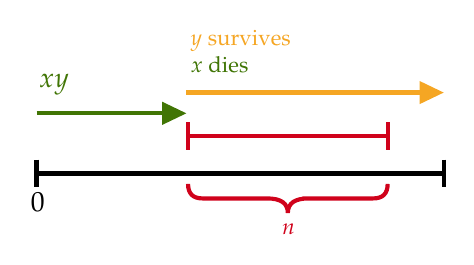
\begin{tikzpicture}[x=0.75pt,y=0.75pt,yscale=-1,xscale=1]
%uncomment if require: \path (0,300); %set diagram left start at 0, and has height of 300

%Straight Lines [id:da6856049917337241] 
\draw [line width=1.5]    (99,119) -- (295.17,119) ;
\draw [shift={(295.17,119)}, rotate = 180] [color={rgb, 255:red, 0; green, 0; blue, 0 }  ][line width=1.5]    (0,6.71) -- (0,-6.71)   ;
\draw [shift={(99,119)}, rotate = 180] [color={rgb, 255:red, 0; green, 0; blue, 0 }  ][line width=1.5]    (0,6.71) -- (0,-6.71)   ;
%Straight Lines [id:da6451112232837601] 
\draw [color={rgb, 255:red, 65; green, 117; blue, 5 }  ,draw opacity=1 ][fill={rgb, 255:red, 245; green, 166; blue, 35 }  ,fill opacity=1 ][line width=1.5]    (99,90) -- (153.17,90) -- (167.17,90) ;
\draw [shift={(171.17,90)}, rotate = 180] [fill={rgb, 255:red, 65; green, 117; blue, 5 }  ,fill opacity=1 ][line width=0.08]  [draw opacity=0] (11.61,-5.58) -- (0,0) -- (11.61,5.58) -- cycle    ;
%Straight Lines [id:da7705877456695056] 
\draw [color={rgb, 255:red, 208; green, 2; blue, 27 }  ,draw opacity=1 ][line width=1.5]    (172.17,101) -- (268.17,101) ;
\draw [shift={(268.17,101)}, rotate = 180] [color={rgb, 255:red, 208; green, 2; blue, 27 }  ,draw opacity=1 ][line width=1.5]    (0,6.71) -- (0,-6.71)   ;
\draw [shift={(172.17,101)}, rotate = 180] [color={rgb, 255:red, 208; green, 2; blue, 27 }  ,draw opacity=1 ][line width=1.5]    (0,6.71) -- (0,-6.71)   ;
%Straight Lines [id:da8192385110842837] 
\draw [color={rgb, 255:red, 245; green, 166; blue, 35 }  ,draw opacity=1 ][line width=1.5]    (171.17,80) -- (225.33,80) -- (291.17,80) ;
\draw [shift={(295.17,80)}, rotate = 180] [fill={rgb, 255:red, 245; green, 166; blue, 35 }  ,fill opacity=1 ][line width=0.08]  [draw opacity=0] (11.61,-5.58) -- (0,0) -- (11.61,5.58) -- cycle    ;
%Shape: Brace [id:dp44682577336929397] 
\draw  [color={rgb, 255:red, 208; green, 2; blue, 27 }  ,draw opacity=1 ][line width=1.5]  (172,124) .. controls (172,128.67) and (174.33,131) .. (179,131) -- (210.08,131) .. controls (216.75,131) and (220.08,133.33) .. (220.08,138) .. controls (220.08,133.33) and (223.41,131) .. (230.08,131)(227.08,131) -- (261.17,131) .. controls (265.84,131) and (268.17,128.67) .. (268.17,124) ;

% Text Node
\draw (95,127) node [anchor=north west][inner sep=0.75pt]   [align=left] {$\displaystyle 0$};
% Text Node
\draw (99,70) node [anchor=north west][inner sep=0.75pt]  [color={rgb, 255:red, 65; green, 117; blue, 5 }  ,opacity=1 ] [align=left] {$\displaystyle xy$};
% Text Node
\draw (172,49) node [anchor=north west][inner sep=0.75pt]  [font=\footnotesize,color={rgb, 255:red, 65; green, 117; blue, 5 }  ,opacity=1 ] [align=left] {\textcolor[rgb]{0.96,0.65,0.14}{$\displaystyle y$ survives}\\\textcolor[rgb]{0.25,0.46,0.02}{$\displaystyle x$ dies}};
% Text Node
\draw (216,142) node [anchor=north west][inner sep=0.75pt]  [font=\footnotesize,color={rgb, 255:red, 208; green, 2; blue, 27 }  ,opacity=1 ] [align=left] {$\displaystyle n$};


\end{tikzpicture}
\end{center}

\end{multicols*}

\pagebreak
\raggedcolumns
\begin{multicols*}{2}
\section{Preuves}
\begin{center}
	\lfbox[rappel]{Preuve de la fonction de densité du couple $(x, y)$}
\end{center}
\begin{formula}{}
\begin{align*}
	f_{T_{x, y}}(t)
	&=	\deriv{t}{F_{T_{x, y}}(t)}	
	\equiv	-\deriv{t}{S_{T_{x, y}}(t)}	\\
	&=	\left(-\deriv{t}{\px[t]{x}}\right) \px[t]{y}	+	\left(-\deriv{t}{\px[t]{y}}\right) \px[t]{x}	\\
	&=	\left(-\deriv{t}{\px[t]{x}}\right) {\color{teal} \times \left( \frac{\px[t]{x}}{\px[t]{x}} \right)} \px[t]{y}	+	\left(-\deriv{t}{\px[t]{y}}\right) {\color{teal} \times \left( \frac{\px[t]{y}}{\px[t]{y}} \right)}\px[t]{x}	\\
	&=	{\color{cyan}\left(\frac{-\deriv{t}{\px[t]{x}}}{{\px[t]{x}}}\right)} \times \px[t]{x} \px[t]{y}	+	{\color{cyan}\left(\frac{-\deriv{t}{\px[t]{y}}}{{\px[t]{y}}}\right)} \times \px[t]{x} \px[t]{y}	\\
	&=	{\color{cyan} \mu_{x + t}} \times {\color{teal}\px[t]{x} \px[t]{y}}	+	{\color{cyan} \mu_{y + t}} \times {\color{teal}\px[t]{x} \px[t]{y}}	\\
	&\overset{T_{x} \perp T_{y}}{=}	\mu_{x + t} \times {\color{teal} \px[t]{xy}} + \mu_{y + t} \times {\color{teal} \px[t]{xy}}	\\
	&=	\px[t]{xy}(\mu_{x + t} + \mu_{y + t})
\end{align*}
\end{formula}


\begin{center}
	\lfbox[rappel]{Preuve de la covariance pour deux vies indépendantes $(x)$ et $(y)$}
\end{center}
\begin{formula}{}
\begin{align*}
	\text{Cov}(v^{T_{\overline{xy}}}, v^{T_{xy}})
	&=	\text{E}[v^{T_{\overline{xy}}}v^{T_{xy}}]	-	{\color{airforceblue}\text{E}[v^{T_{\overline{xy}}}]\text{E}[v^{T_{xy}}]}	\\
	&=	\text{E}[v^{\color{teal}T_{\overline{xy}} + T_{xy}}]	-	{\color{airforceblue}\Ax*{\overline{xy}}\Ax*{xy}}	\\
	&=	\text{E}[v^{\color{teal}T_{x} + T_{y}}]	-	\Ax*{\overline{xy}}\Ax*{xy}	\\
	&\overset{T_{x}\perp T_{y}}{=}	{\color{airforceblue}\text{E}[v^{T_{x}}]\text{E}[v^{T_{y}}]}	-	\Ax*{\overline{xy}}\Ax*{xy}	\\
	&=	{\color{airforceblue}\Ax*{x}\Ax*{y}}	-	{\color{teal}\left(\Ax*{\overline{xy}}\right)}\Ax*{xy}	\\
	&=	\Ax*{x}\Ax*{y}	-	{\color{teal}\left(\Ax*{x} + \Ax*{y} - \Ax*{xy}\right)}\Ax*{xy}	\\
	&=	\Ax*{x}(\Ax*{y}	-	\Ax*{xy})	-	\Ax*{xy}(\Ax*{y}	-	\Ax*{xy})	\\
	&=	(\Ax*{x}	-	\Ax*{xy})(\Ax*{y}	-	\Ax*{xy})	\\
\end{align*}
\end{formula}


\end{multicols*}
\end{document}

